\documentclass[../main.tex]{subfiles}
\begin{document}
\subsection{Условие применимости метода линеаризации в задаче локального синтеза} 

\subsubsection{Постановка задачи}

Рассмотрим нелинейную систему, аффинную по управлению:
\begin{gather}\label{s22:nonlinear}
 \dot{z}(t)=f(z(t))+B u(t),\qquad 0 \leqslant t \leqslant T, \qquad z(0) = z_0,
\end{gather}
 где $ z \in \mathbb{R}^n $ --- вектор состояния, $ u \in \mathbb{R}^r $ --- вектор управления, $B \in \mathbb{R}^{n \times r}$, а $ 
T$ --- некоторое положительное число. 

Система \eqref{s22:nonlinear} является частным случаем системы \eqref{s1:common_nonlinear}, которая исследовалась в Главе~\ref{s1}, при $f_1\big(t,z(t)\big) = f\big(z(t)\big)$ и $f_2\big(t,z(t)\big) = B$. 

Пространство скалярных или векторных функций, интегрируемых с квадратом на $ [0,T] $ будем обозначать здесь через $ \mathbb{L}_2 = \mathbb{L}_2[0,T] $. 

Предполагается, что управление $u(\cdot)$ принадлежит пространству $\mathbb{L}_2 $.
\begin{assumption}\label{s22:as:solution_bounded}
	Существует такое $\mu > 0$, что все решения $x(s, \upsilon(\cdot))$ системы \\ \mbox{$\dot{x} = -f(x)-B\upsilon(t)$}, выходящие из некоторой окрестности нуля и отвечающие управлениям $\upsilon(\cdot) \in B_{\mathbb{L}_2}(0, \mu)$, определены на интервале $[0, T]$ и лежат в шаре $ B_{\mathbb{R}^n}(0,\overline{r})$, $\overline{r} > 0$.
\end{assumption}
Здесь $ B_{\mathbb{R}^n}(0,\overline{r}) $ --- шар радиуса $\overline{r}$ с центром в точке $0 \in \mathbb{R}^n$. 
Будем считать, что функция $f$ обладает следующим свойством.

\begin{assumption}\label{s22:as:Residial_term_bounds}
 Найдутся такие $\overline{r} > r >0$, $k>0$, что при всех $ z \in B_{\mathbb{R}^n}(0,r) $ функция $f(z)$ может быть представлена в форме $ f(z) = Az + R(z) $, причём $A \in \mathbb{R}^{n \times n}$ и $ \|R(z) \| \leqslant k \| z\|^2 $. 
\end{assumption}
Это свойство выполняется, если $f(0) = 0 $, $\frac{\partial f}{\partial z}(0) 
= A $ и  функция $f(z)$ дважды непрерывно дифференцируема. 

Заметим, что из справедливости Предположения \ref{s22:as:Residial_term_bounds} для $f$ следует выполнение условий Предположения \ref{s1:as:right_hand_side_diff_lip} на интервале $ 0 \leqslant t \leqslant T$ в области $B_{\mathbb{R}^n}(0,r)$.

В качестве функционала рассматриваем 
\begin{gather}\label{s22:cost}
 I(T,u):=\int_0^Tu^\top (t)u(t)dt= \lVert u(\cdot)\rVert^2_{\mathbb{L}_2.} 
\end{gather}
Задача состоит в синтезе закона управления $u(t)=u(t,z(t))$, который бы приводил траектории замкнутой системы 
\begin{gather*}
 \dot{z}(t)=f(z(t))+B u(t,z(t)),\qquad 0 \leqslant t \leqslant T, \qquad z(0) = z_0.
\end{gather*}
в начало координат за время $T$ и обеспечивал при этом минимальное значение $I(T,u)$. 

Рассмотрим линейный случай ($R(z)=0$)
\begin{gather}\label{s22:linear}
 \dot{z} = A z + B u, \qquad 0 \leqslant t \leqslant T.
\end{gather}

Если система \eqref{s22:linear} управляема, то решение описанной выше задачи --- это линейный по состоянию закон управления 
\begin{gather}\label{s22:linear_feedback}
 u(t,z) = -B^{\top} Q_T(t) z
\end{gather}
(см., например, \cite{Abgar,Kur1,GusevOsipov}).
Здесь $Q_T(t)=W^{-1}(T-t)$, а $W(t)$ --- грамиан управляемости системы $\dot{x} = -A x - B u$:
\begin{gather*}
 W(t) = \int_0^t e^{-A\tau}BB^\top e^{-A^{\top}\tau}d\tau. 
\end{gather*}

Грамиан $W(t)$ положительно определён при $t>0$ тогда и только тогда, когда 
система \eqref{s22:linear} управляема. 
Можно показать, что $Q_T(t)$ --- решение дифференциального уравнения 
\begin{gather}\label{s22:eqQ}
 \dot{Q_T} = Q_T B B^{\top} Q_T - A^{\top}Q_T - Q_T A, \quad Q_T(0)=W^{-1}(T).
\end{gather}

Таким образом, чтобы найти $Q_T(t)$ на $(0,T]$, нужно сначала вычислить $W(T)$, а затем проинтегрировать систему \eqref{s22:eqQ}.
Поскольку $W(0)=0$, $Q_T(t)$ определена для $t<T$ и $\|Q_T(t)\| \to \infty$ при $t\to T$. 

Верно следующее утверждение \cite{Abgar,Kur1,GusevOsipov}.
\begin{utv}
Любая траектория $z(t)$ системы \eqref{s22:linear} с управлением \eqref{s22:linear_feedback}, выходящая из точки $ z_0 $, достигает начала координат за время $T$. 
При этом интегральный функционал $I(T,u)$ принимает минимальное значение $z^{\top}_0 Q_T(0) z_0 $ при каждом $z_0$.
\end{utv}
Далее мы будем исследовать поведение траекторий системы \eqref{s22:nonlinear} замкнутой линейной обратной связью $ u(t,z) = -B^{\top} Q_T(t) z$ при условии, что $T$ достаточно мало. 
Верно ли, что все траектории, начинающиеся в некоторой окрестности начала координат, достигают его? 
Можно ли что-то сказать о значении интегрального функционала? 

\subsubsection{Асимптотическая эквивалентность множеств достижимости}

Будем использовать понятие асимптотической эквивалентности множеств, введённое в разделе \ref{sec21:AsymptoticEquality}. 
Рассмотрим систему, уравнения которой получаются из \eqref{s22:nonlinear} обращением времени. 
Положив $\tau=T-t$, имеем
\begin{gather}\label{s22:nonlinear_}
 \dot{x}(\tau)=-f(x(\tau))-B v(\tau),\qquad 0 \leqslant \tau \leqslant T,
\end{gather}
где $x(\tau)=z(T-\tau)$, $v(\tau)=u(T-\tau)$.
При заданном $\mu>0$ обозначим через $ G_{-} (T,\mu)$ множество достижимости системы \eqref{s22:nonlinear_} с интегральными квадратичными ограничениями на управление: $G_{-}(T,\mu)=\{x\in \mathbb{R}^n:\exists v(\cdot)\in B_{\mathbb{L}_2}(0,\mu),\; x=x( T,v(\cdot))\}$.
 
Здесь $x( \tau,v(\cdot))$ обозначает решение системы \eqref{s22:nonlinear_} с нулевыми начальными условиями. 
Свойства множеств достижимости нелинейных систем с интегральными ограничениями на управление изучались во многих работах (см., например, \cite{Guseinov2010,Rousse,GusZykIFAC}).
Рассмотрим также линейную систему 
\begin{gather}\label{s22:linear_}
 \dot{x}(\tau)=-Ax(\tau)-B v(\tau),\qquad 0 \leqslant \tau \leqslant T,
\end{gather}
которая является линеаризацией системы \eqref{s22:nonlinear_} в начале координат. 
Множество достижимости этой системы обозначим через $G_{-}^0(T,\mu)$. 
Это множество --- эллипсоид в $\mathbb{R}^n$, описываемый соотношением $G_{-}^0(T,\mu)=\{x \in \mathbb{R}^n: x^\top W^{-1}(T)x\leqslant \mu^2\}$. 

%Let $X,Y \subset \mathbb R^n $ be convex compact sets such that the origin is an interior point of both the sets.
%\begin{definition}[see, for example, \cite{Lassak,Ovs}]
%The Banach-Mazur distance between $X$ and $Y$ is defined as
%$\rho(X,Y):=\log\big(r(X,Y)\cdot r(Y,X)\big)$, where \\ $r(X,Y)=\inf \{t\geqslant1:tX \supset Y\}$. 
%\end{definition} 
%From the definition it follows that for any $c>0$, $\rho(cX,cY)=\rho(X,Y)$ and two inclusions are valid: $X\subset \exp(\rho(X,Y))Y$ and $Y\subset \exp(\rho(X,Y))X$.

%Assume that $X,Y$ depend on a small positive parameter $\tau$, $0<\tau\leqslant\tau_0$ and set-valued mappings $X(\tau), Y(\tau)$ are bounded. 
%\begin{definition}[\cite{Ovs}] 
% The sets $ X (\tau), Y (\tau) $ are called asymptotically equal under $\tau \to 0$ if $ \rho (X (\tau), Y (\tau)) \to 0,\;\; \tau \to 0$.
%\end{definition}
Через $\nu(\tau), \eta(\tau)$ обозначим наименьшее и наибольшее собственное число $W(\tau)$ соответственно. 
Из результатов \cite{Polyak2001,GusevOsipovTrudy,Osipov,GusevMotor} следует, что множества достижимости 
$G_{-}(\tau,\mu)$ и $G_{-}^0(\tau,\mu)$ асимптотически эквивалентны при $\tau \to 0$, если пара $(A,B)$ управляема 
и существуют такие $ l > 0$, $\tau_0 > 0$ и $\alpha > 0$, что для всех $0 < \tau \leqslant \tau_0 $ выполнено неравенство
 \begin{gather}\label{s22:gramas}
 \nu(\tau)\geqslant l\tau^{4-\alpha}.
 \end{gather}

\begin{zam}
 Множество достижимости $G_{-}(T,\mu)$ системы \eqref{s22:nonlinear_} совпадает с множеством нуль-управляемости системы \eqref{s22:nonlinear}, т.~е. множеством таких начальных состояний, из которых система может быть переведена в начало координат управлениями из $B_{\mathbb{L}_2}(0,\mu) $ за время $T$. 
 То же самое справедливо для систем \eqref{s22:linear} и \eqref{s22:linear_} и соответствующих им множеств $G_{-}^0(T,\mu)$.
\end{zam}

\subsubsection{Задача синтеза управления. Асимптотика траекторий}

Далее будем предполагать, что пара $(A,B)$ является управляемой, не уточняя это отдельно.

В этом разделе исследуем асимптотическое поведение траекторий системы \eqref{s22:nonlinear}, замкнутой линейной обратной связью $ u(t,z) = -B^{\top} Q_T(t) z$:
\begin{gather}\label{s22:nonlinear_closed}
 \dot{z} = f(z) - B B^{\top} Q_T(t) z, \qquad 0 \leqslant t \leqslant T, \qquad z(0) = z_0.
\end{gather}
Напомним, что это управление приводит траектории линейной системы $\dot{z} = A z + B z$ к началу координат в момент времени $T$ и обеспечивает минимальное значение функционала. 
Это значение равно $J_0(T,z_0) =z_0^{\top}Q_T(0)z_0$.

Для анализа траекторий системы \eqref{s22:nonlinear_closed} используем следующую лемму.
\begin{lemma}\label{s22:lem:zqz} 
 Пусть $C\in \mathbb{R}^{ n \times n}$ и $D\in \mathbb{R}^{n \times n}$ --- симметричные положительно-определенные матрицы, $C=D^{-1}$. 
Тогда для любого $\forall z \in \mathbb{R}^{n}$ выполнены неравенства
 \begin{gather} \label{s22:eig}
 \frac{1}{\lambda_{\max}(D)} \|z\|^2 \leqslant z^T C z \leqslant \frac{1}{\lambda_{\min}(D)} \|z\|^2,
 \end{gather}
 где $\lambda_{\max}(D)$ и $\lambda_{\min}(D)$ --- наибольшее и наименьшее собственные числа матрицы $D$.
\end{lemma}
\doc 
 Следует из факта, что наибольшее и наименьшее собственное число матрицы $C$ равны $1/{\lambda_{\min}(D)}$ и $1/{\lambda_{\max}(D)}$, соответственно. \hfill $ \square $

Если $C=Q_T(t)=W^{-1}(T-t)$, то $D=W(T-t)$ и неравенство \eqref{s22:eig} принимает вид
\begin{gather*} %\label{s22:eig1}
 \frac{1}{\eta(T-t)} \|z\|^2 \leqslant z^T Q_T(t) z \leqslant \frac{1}{\nu(T-t)} \|z\|^2, \quad 0\leqslant t < T.
 \end{gather*}
\begin{assumption} \label{s22:asm1} 
 Пусть существуют $\overline{T}>0$ и непрерывная положительная функция $\varphi(\tau): (0, \overline{T}] \to \mathbb{R}$ такие, что
\begin{gather*}
 0 < \frac{\eta(\tau)}{\sqrt{\nu(\tau)}} \leqslant \varphi(\tau), \qquad 0 < \tau \leqslant \overline{T},\quad \int\limits_0^ {\overline{T}}\varphi(\tau) d\tau<\infty.
\end{gather*} 
\end{assumption}
Введём функцию $\Phi(T): [0, \overline{T}] \to \mathbb{R}$
\begin{gather*}
 \Phi(T)= \int\limits_0^ {T}\varphi(\tau) d\tau,\quad 0 < T \leqslant \overline{T},\quad \Phi(0)=0.
\end{gather*} 

Напомним, что $\nu(\tau)$ и $\eta(\tau)$  --- это наименьшее и наибольшее собственные числа $W(\tau)$. 
Далее будем считать систему \eqref{s22:linear_} полностью управляемой, поэтому $\eta(\tau) \geqslant \nu(\tau) \geqslant 0$ при $\tau \geqslant 0$.
 
Поскольку $\varphi(\tau)$ не обязательно ограничено в нуле, $\Phi(T)$ может принимать значения, равные $+\infty$.
\begin{lemma}%\label{s22:lem:Phi}
Верны следующие свойства $\Phi(T)$:
\begin{enumerate}
 \item Если $\Phi(T) < \infty $ хотя бы для одного $T$, то $\Phi(T) < \infty $ для всех $T \in (0, \overline{T}]$.
\item Если $\Phi(T) < \infty $, то $\Phi(T)$ непрерывная и возрастающая функция на $ [0,\overline{T}]$.
 \end{enumerate}
\end{lemma}
\doc 
Следует из свойств несобственных интегралов. \hfill $ \square $
\begin{assumption}\label{s22:asm2}
Существует такое $ 0 < \beta \leqslant 1$, что $\frac{\sqrt{\eta(T)}}{\Phi^\beta(T)} \to 0$ при $T \to 0$.
\end{assumption}
Если $\Phi(T)$ конечна, то существует не более одного корня уравнения $\Phi(T)=1$ на $(0,\overline{T}]$, обозначим этот корень через $\check{T}$. 
Если $\Phi(T)<1$ при $T\in (0,\overline{T}]$, положим $\check{T}=\overline{T}$. 
Очевидно, что для всех $ 0 < \beta \leqslant 1$ выполнено неравенство $\Phi^\beta(T)\geqslant \Phi(T)$ если $T \leqslant \check{T}$.

При фиксированном $T\in (0, \overline{T}]$ рассмотрим квадратичную форму $V_T(t,z)=z^{\top}Q_T(t)z$. 
\begin{lemma}\label{s22:lem:vest}
 Пусть выполнено предположение \ref{s22:asm1}. 
Если $T\leqslant \check{T}$ и $z(t)$ --- такая траектория системы \eqref{s22:nonlinear_closed}, что $z(t) \in B(0,r)$ при $0<t \leqslant T$ и $V_T(0,z(0))\leqslant 1/(4k^2\Phi^{2\beta}(T))$ для некоторого $0<\beta \leqslant 1$, то
 \begin{gather*}
 V_T(t,z(t)) \leqslant \frac{1}{k^2\Phi^{2\beta}(T)}, \qquad 0 \leqslant t \leqslant T. 
 \end{gather*}
\end{lemma}
\doc 
Продифференцировав $V_T$ вдоль траектории $z(t)$ системы \eqref{s22:nonlinear} на интервале $[0, T]$, получим
\begin{gather*}
 \frac{d}{dt}V_T(t,z) = \frac{d}{dt}z^{\top}Q_Tz = \dot{z}^{\top} Q_T z + z^{\top} \dot{Q_T} z + z^{\top} Q_T \dot{z} = \\
 =\left(z^{\top} A^{\top} + R^{\top}(z)- z^{\top} Q_T B B^{\top}\right) Q_T z + \\ +
 z^{\top} Q_T \left(A +R(z) - B B^{\top} Q_T\right)z + z^{\top} \left(Q_T B B^{\top} Q_T - A^{\top}Q_T - Q_T A \right) z = \\
 = R^{\top}(z)Q_T z + z^{\top} Q_T R(z) - z^{\top} (Q_T B B^{\top} Q_T) z = \\
 = 2 \left( R(z), Q_Tz \right) - z^{\top} Q_T B B^{\top} Q_T z.
\end{gather*}
Хотя здесь $z$ и $Q_T$ зависят от $t$, для краткости мы опускаем явную зависимость в обозначениях. 
Из $z^{\top} Q_T B B^{\top} Q_T z\geqslant 0$, следует, что
\begin{gather}\label{s22:dvt_first}
 \frac{d}{dt}V_T(t,z) \leqslant 2 \left( R(z), Q_T z\right)=2(R(z),z)_{Q_T} \leqslant 2 \| R(z) \|_{Q_T} \| z \|_{Q_T}.
\end{gather}
Здесь использованы обозначения $(x,y)_{Q_T}=x^\top Q_Ty$ и $\| x \|_{Q_T} =\sqrt{(x,x)_{Q_T}}$ для $x,y\in \mathbb R^n$. 
Так как $z = z(t) \in B(0,r)$, то, учитывая, что $\|R(z)\| \leqslant k\|z\|^2$ и применяя Лемму \ref{s22:lem:zqz}, получаем 
\begin{gather}\label{s22:rqr_est}
 \| R(z) \|_{Q_T} \leqslant \frac{1}{\sqrt{\nu(T - t)}} \|R(z)\| \leqslant \frac{k}{\sqrt{\nu(T - t)}}\|z\|^2 \leqslant k \frac{\eta(T-t)}{\sqrt{\nu(T-t)}}V_T.
\end{gather}
Напомним, что $ Q_T^{-1}(t) = W(T-t) $.
Подставляя полученную выше оценку в \eqref{s22:dvt_first}, приходим к оценке
\begin{gather}\label{s22:dvt}
 \frac{d}{dt}V_T \leqslant 2 k \frac{\eta(T-t)}{\sqrt{\nu(T-t)}}V_T^{\frc{3}{2}} \leqslant 2k \varphi(T-t) V_T^{\frc{3}{2}}.
\end{gather}
Введём систему
\begin{gather}\label{s22:comparison_system}
 \dot{\psi} = 2k \varphi(T-t) \psi,
\end{gather}
которую будем использовать как систему сравнения для \eqref{s22:dvt}. 
Проинтегрировав эту систему, мы имеем
\begin{gather*}
 d\psi^{-\frc{1}{2}} = -k \varphi(T-t) dt, \quad
 \psi^{-\frc{1}{2}}(t) = -k \int\limits_0^t \varphi(T-\zeta) d\zeta + C,
\end{gather*}
где
\begin{gather*}
 0 < \int\limits_0^t \varphi(T-\zeta) d\zeta \leqslant \int\limits_0^T \varphi(T-\zeta) d\zeta = 
 \int\limits_0^T \varphi(\tau) d\tau = \Phi(T).
\end{gather*}
Выберем $C = 2k (\Phi(T))^{\beta}$, тогда $\psi^{-\frc{1}{2}} \geqslant 2k (\Phi(T))^{\beta} - k \Phi(T) = k (2\Phi^\beta - \Phi)\geqslant k\Phi^\beta $.
%% \\ \frac{2\Phi^\beta - \Phi}{\Phi} = 2 - \Phi^{1 - \beta} \to 2, \mbox{ while } \Phi \to 0 
Поэтому $\psi(t) \leqslant \big(k^2\Phi^{2\beta}(T)\big)^{-1}$ для всех $ 0 \leqslant t \leqslant \check{T} $ и $\psi(0) = \big(4k^2\Phi^{2\beta}(T)\big)^{-1} $.
Таким образом, \mbox{$V_T(0,z(0))\leqslant \psi(0)$}, и теорема сравнения \cite{walter}, применённая к \eqref{s22:dvt}, \eqref{s22:comparison_system}, означает, что выполняется неравенство $V_T(t,z(t))\leqslant \psi(t)$. 
Это завершает доказательство.
 \hfill $ \square $

\begin{theorem}\label{s22:th:tends_to_zero}
 Пусть выполнены предположения \ref{s22:asm1}, \ref{s22:asm2}. 
Тогда существует момент $ T_1 \leqslant \check{T}$, что для всех $ T \leqslant T_1$ найдётся такое $ r_1(T)$, что траектории системы \eqref{s22:nonlinear_closed}, выходящие из $z(0) = z_0 \in B(0,r_1(T))$, стремятся к $0$ при $t \to T$.
\end{theorem}

\doc 
Поскольку $\frac{\sqrt{\eta(T)}}{\Phi^\beta(T)} $ стремится к $0$, если $T$ стремится к $0$, то найдётся момент $ T_1 \leqslant \check{T}$, что выполняется следующее неравенство:
$ \sqrt{\eta(T)}/(k\Phi^\beta(T)) \leqslant r/{2}$, $ \forall T \in [0;T_1]$.

Определим $r_1(T)$ равенством
\begin{gather}\label{s22:r1}
 r_1(T) = \min \left\{ \frac{r}{4}, \frac{\sqrt{\nu(T)}}{2k\Phi^\beta(T)} \right\}.
\end{gather}


Нам нужно доказать, что вся траектория $z(t)$ лежит в шаре $B(0,r)$, чтобы использовать оценку \eqref{s22:z_est} из предыдущего раздела. 
Из \eqref{s22:r1} немедленно следует, что $r_1(T) < r$. 
Отсюда и из условий теоремы получаем, что $z_0 \in B(0,r_1(T)) \subset B(0,r) $. 
Более того, непрерывность траектории $z(t)$ означает, что условие $z(t) \in B(0,r) $ выполняется и для близких к нулю значений $t$. 

Обозначим $\check{t} = \sup \left\{ t: z(t) \in B\left(0,0.5r\right)\right\} $.
Предположим, что $\check{t} < T$.
Это означает, что $z(t) \notin B(0,0.5r)$ при $t > \check{t}$. 
Тогда мы можем выбрать такое положительное $ \varepsilon$, что включение $z(t) \in B(0,r)$ будет выполняться для всех $0 \leqslant t \leqslant \check{t} + \varepsilon$. 

Из условия \eqref{s22:r1} следует, что для $0 \leqslant t \leqslant \check{t} + \varepsilon$ будет выполняться следующее условие:
\begin{gather*}
 V_T(0,z_0) \leqslant \frac{1}{\nu(T)} \|z_0\|^2 \leqslant \frac{1}{\nu(T)} r_1^2 \leqslant \frac{1}{4k^2\Phi^{2\beta}(T)}.
\end{gather*}
Из Леммы \ref{s22:lem:vest} вытекает, что 
$V_T(t, z(t)) \leqslant \psi(t) $ и
\begin{gather}\label{s22:z_est}
 \|z(t)\|^2 \leqslant \eta(T-t) V_T(t,z(t)) \leqslant \eta(T-t) \psi(t) \leqslant \frac{\eta(T)}{k^2\Phi^{2\beta}(T)}.
\end{gather}
Поэтому $\|z(t)\| \leqslant \frac{\sqrt{\eta(T)}}{k\Phi^\beta(T)} \leqslant r/2$ для всех $0\leqslant t \leqslant \check{t}+\varepsilon$,
что противоречит определению $\check{t}$. 
Следовательно, включение $z(t) \in B(0,r) $ и неравенство $V_T(t,z(t)\leqslant \psi(t)$ справедливы для всех $t \in [0; T]$.
 
Наконец, $ \|z(t)\|^2 \leqslant \eta(T-t)\psi(t) \leqslant \eta(T-t)\big(k^2\Phi^{2\beta}(T)\big)^{-1} $, 
где $\eta(T-t) \to 0$ при $t \to T$.
 Это означает, что $\|z(t)\|$ тоже стремится к нулю.
 \hfill $ \square $
\begin{corollary}%\label{s22:cor:1}
Пусть существуют такие $ l > 0$, $\tau_0 > 0$ и $\alpha > 0$, что для всех $0 < \tau \leqslant \tau_0 $ выполняется неравенство
 \begin{gather}\label{s22:asymp}
 \nu(\tau)\geqslant l\tau^{4-\alpha}.
 \end{gather}
 Тогда справедливы Предположения \ref{s22:asm1} и \ref{s22:asm2} и, следовательно, утверждение Теоремы \ref{s22:th:tends_to_zero} является верным.
\end{corollary}
\doc 
Положим $\overline{T}=\tau_0$. 
Существует такое $m>0$, что $\eta(\tau)\leqslant m \tau$ для $0 < \tau \leqslant\overline{T}$ (см., например, \cite{GusevOsipov}). 
Следовательно, имеем $
\eta(\tau)/\sqrt{\nu(\tau)} \leqslant 
 ml^{-1/2}\tau^{-1+\alpha/2},$
и можем взять $\varphi(\tau):= 
 ml^{-1/2}\tau^{-1+\alpha/2}$. 
В этом случае 
$\Phi(T)=2mT^{\alpha/2}/(l^{-1/2}\alpha)$, и Предположение \ref{s22:asm1}, очевидно, выполняется. 
Поскольку 
$\sqrt{\eta(T)}/\Phi^\beta(T) \leqslant c_0T^{(1-\alpha\beta)/2},$
где $c_0$ --- константа, то для выполнения Предположения \ref{s22:asm2} достаточно взять $\beta < 1/\alpha$.
 \hfill $ \square $
 
 
Заметим, что неравенство \eqref{s22:asymp} совпадает с условием, из которого следует Теорема 1 из \cite{GusevOsipov}.

\subsubsection{Оценка погрешностей в значениях функционала}

В этой части работы сосредоточимся на значении интегрального функционала \eqref{s22:cost} при применении линейной обратной связи \eqref{s22:linear_feedback} к нелинейной системе \eqref{s22:nonlinear}.
Напомним, что в линейном случае системы \eqref{s22:linear} этот функционал принимает минимальное значение на управлении \eqref{s22:linear_feedback}.
Ранее мы обозначили это значение через $J_0(T,z_0)$.
Обозначение $J(T,z_0)$ мы используем для значения функционала на траектории системы \eqref{s22:nonlinear_closed}. 
Для того, чтобы получить выражение для $J(T,z_0)$ нужно проинтегрировать \eqref{s22:dvt_first} от $0$ до $t$:
\begin{gather}\label{s22:J}
 z^{\top}(t) Q_T(t)z(t) = z_0^{\top} Q_T(0)z_0 - \int_{0}^{t} u^{\top}(\xi) u(\xi) \, d\xi + 2\int_{0}^{t} R^{\top}(z(\xi))Q_T(\xi) z(\xi) d\xi,
\end{gather}
 где $ u(\xi) = -B^{\top} Q_T(\xi) z(\xi)$ --- управление в момент времени $\xi$. 
В линейном случае, $R(z) \equiv 0$ и $z^{\top}(t) Q_T(t)z(t) \to 0 $ при $t \to T$, так что
\begin{gather*}
 J_0(T,z_0) = z_0^{\top} Q_T(0)z_0 = \int_{0}^{t} u^{\top}(\xi) u(\xi) \, d\xi.
\end{gather*}
Далее мы собираемся исследовать поведение квадратичной формы $z^{\top}(t) Q_T(t)z(t) $ и остаточного члена в \eqref{s22:J}, который обозначим через
\begin{gather*}
 \gamma (t,z_0) = 
 2\int_{0}^{t} R^{\top}(z(\xi,z_0))Q_T(\xi) z(\xi,z_0) d\xi.
\end{gather*}

\begin{theorem}\label{s22:th:functional_error_estimate}
 Пусть выполнено предположение \ref{s22:asm1}. 
Пусть $x(t)$ --- такая траектория системы \eqref{s22:nonlinear_closed}, что $x(t)\in B(0,r)$ при $0\leqslant t \leqslant \tilde{T} \leqslant \overline{T} $ и $V_{\tilde{T}}(t,x(t))\to 0$ при $t\to \tilde{T}$. 
 Тогда существует такое $T_2 \leqslant \tilde{T}$, что для всех $0 < T < T_2 $ выполняется следующая оценка:
 \begin{gather} \label{s22:est}
 \left| \frac{ J(T) - J_0(T)}{J_0(T)}\right| \leqslant 16k\Phi({T})J^{1/2}_0(T).
 \end{gather}
 Здесь $J(T)=J(T,x(\tilde{T}-T))$, $J_0(T)=J_0(T,x(\tilde{T}-T))$ --- значения функционала $I(T,u(\cdot))$ на траекториях нелинейной и линеаризованной систем соответственно.
\end{theorem}
\doc 
Пусть $T\leqslant \tilde{T}$. 
Через $z(t)$ обозначим траекторию системы \eqref{s22:nonlinear_closed} с начальным условием $z(0)=x(\tilde{T}-T)$ и определённую на интервале $[0,T)$. 
Тогда имеем 
\begin{gather*}
Q_T(t)=W^{-1}(T-t)=W^{-1}(\tilde{T}-(\tilde{T}-T+t))=Q_{\tilde{T}}(\tilde{T}-T+t) = Q_T(\tau), \\ 
V_T(t,z(t))=z^\top(t)Q_T(t)z(t)=V_{\tilde{T}}(\tau,x(\tau)),
\end{gather*}
где $\tau=\tilde{T}-T+t$,  
$V_T(0,z(0))=V_{\tilde{T}}(\tilde{T}-T, x(\tilde{T}-T))$, $V_{\tilde{T}}(t,x(t))\to 0$ при $t\to \tilde{T}$. 
Поскольку $V_{\tilde{T}}(t,x(t))\to 0$, $t\to \tilde{T}$, мы получаем, что $V_T(0,z(0))=J_0(T)$ стремится к нулю при $T\to 0$.
Ясно, что $V_T(t,z(t))=z^\top(t)Q_T(t)z(t)=V_{\tilde{T}}(\tau,x(\tau))$ стремится к нулю при $t\to T$.
Используя это, перепишем \eqref{s22:J} в виде
\begin{gather}\label{s22:J1}
 \int_{0}^{T} u^{\top}(\xi) u(\xi) \, d\xi - z_0^{\top} Q_T(0)z_0= 2\int_{0}^{T} R^{\top}(z(\xi))Q_T(\xi) z(\xi) d\xi=\gamma(T,z(0)),
\end{gather}
и изучим подробнее подынтегральное выражение $\left( R(z), Q_T z\right)=(R(z),z)_{Q_T} \leqslant \| R(z) \|_{Q_T} \| z \|_{Q_T}$.
Повторяя шаги \eqref{s22:rqr_est}, \eqref{s22:dvt} из доказательства леммы \ref{s22:lem:vest}, приходим к следующей оценке сверху:
\begin{gather}\label{s22:rqz}
 2 \left( R(z), Q_T z\right) \leqslant 2 k \frac{\eta(T-t)}{\sqrt{\nu(T-t)}}V_T^{\frc{3}{2}} \leqslant 2k \varphi(T-t) V_T^{\frc{3}{2}},
\end{gather}
которая аналогична \eqref{s22:dvt}. 
Однако дальнейшие действия с системой сравнения здесь несколько изменены. 
Интегрируя систему сравнения $\dot{\psi} = 2k \varphi(T-t)\psi$, имеем
\begin{gather*}
 d\psi^{-\frc{1}{2}} = -k \varphi(T-t) dt, \quad
 \psi^{-\frc{1}{2}}(t) = -k \int\limits_0^t \varphi(T-\zeta) d\zeta + C.
\end{gather*}
Поскольку $V_T(0,z(0))\to 0$ и $\Phi(T) \to 0$ при $T\to 0$, то найдётся такое $T_2$, что при всех $T\leqslant T_2$ выполняется неравенство $\Phi(T) \sqrt{V_T(0,z(0))} \leqslant 1/2k$. 
Переписав это неравенство, получаем
\begin{gather*}
 \frac{1}{2\sqrt{V_T(0,z(0))}} \geqslant k\Phi(T).
\end{gather*} 
Выберем $C = 1/\sqrt{V_T(0,z(0))}$.
Тогда
 \begin{gather*}
\psi^{-\frc{1}{2}}(t) = -k \int\limits_0^t \varphi(T-\zeta) d\zeta + C\geqslant -k\Phi(T)+C\geqslant \frac{1}{2\sqrt{V_T(0,z(0))}}.
\end{gather*} 
Следовательно, $\psi(t) \leqslant 4V_T(0,z(0))=4J_0(T)$. 
Поскольку $\psi(0)=V_T(0,z(0))$, из теоремы сравнения получаем, что $V_T(t,z(t))\leqslant \psi(t) \leqslant 4J_0(T)$ при $ 0\leqslant t <T$.

Подставляя эту оценку в \eqref{s22:rqz}, мы получаем $\left( R(z), Q_T z\right) \leqslant k \varphi(T-t) \left( 4J_0(T) \right) ^{\frc{3}{2}} $.
Теперь остаётся только проинтегрировать это выражение и использовать его в \eqref{s22:J1}:
\begin{gather*}
J(T)-J_0(T)= \gamma (T,z(0)) = 
 2\int_{0}^{T} R^{\top}(z(\xi))Q_T(\xi) z(\xi) d\xi\leqslant 2k \Phi(T) (4J_0(T))^{3/2}, 
\end{gather*}
откуда и следует \eqref{s22:est}.
 \hfill $ \square $ \\
 
Так как при предположениях Теоремы \ref{s22:th:functional_error_estimate} $\Phi(T)$ и $J_0(T)$ стремятся к нулю, то правая часть \eqref{s22:est} тоже стремится к нулю при $T\to 0$.

В теореме \ref{s22:th:tends_to_zero} мы доказали, что траектория $z(t)$ системы \eqref{s22:nonlinear_closed} стремится к нулю при $t\to T$ и $V_{T}(t,z(t))$ ограничена в окрестности $T$. 
Следующая теорема даёт условия, при которых $V_{T}(t,z(t))\to 0$ при $t\to T$.
\begin{theorem}
 Пусть выполнено неравенство \eqref{s22:gramas}. 
Пусть $T \leqslant \overline{T}$ и траектория $z(t)$ системы \eqref{s22:nonlinear_closed} стремится к нулю при $t\to T$. 
Тогда $V_{T}(t,z(t)) =z^{\top}(t)Q_T(t)z(t) \to 0$ при $t \to T$.
\end{theorem}
%\textbf{An alternative formulation of theorem 3}. {\it Let all the following statements be true.
%\begin{enumerate}
 %\item Assumption \ref{s22:asm1} is valid.
 %\item The trajectory $z(t)$ of system\eqref{s22:nonlinear_closed} tends to zero as $t\to T$.
 %\item $T$ is not greater than $\check{T}$.
 %\item $V_T(0,z(0))\leqslant 1/(4k^2\Phi^{2\beta}(T))$ for some $0<\beta \leqslant 1$.
 %\item $z(t) \in B(0,r) $ for all $t \in (0,T] $.
 %\item The smallest eigenvalue of the Gramian of system \eqref{s22:linear_} satisfy the inequality \eqref{s22:gramas} for all $\tau \in (0, %\tau_0] $, where $\tau_0$ is a positive number.
%\end{enumerate} Then $V_{T}(t,z(t)) = z^{\top}(t)Q_T(t)z(t) $ tends to $ 0$ as $t $ tends to $T$.} 
\doc 
Заметим, что функция $ u(\xi) = -B^{\top} Q(\xi) z(\xi)$  непрерывна на интервале $0 \leqslant \xi <T$. 

Также заметим, что функция $V_{T}(t,z(t))$ может не быть ограниченной только в окрестности точки $t = T$. 
% However, taking into account that the fulfillment of the inequality \eqref{s22:gramas} implies the fulfillment of the assumption, one can see that it follows from $z(t) \to 0 $ that the conditions of lemma \ref{s22:lem:vest} will be met for $t$ from the neighborhood of $T$.
Однако, учитывая, что выполнение неравенства \eqref{s22:gramas} предполагает выполнение условия теоремы, можно увидеть, что из $z(t)\to 0 $ следует, что условия леммы~\ref{s22:lem:vest} будут выполняться для $t$ из окрестности $T$.
Следовательно, $V_{T}(t,z(t))$ ограничена на всей траектории $z(t)$. 
Теперь из соотношения \eqref{s22:J} видно, что интегральная величина $I(t,u) = \int_{0}^{t} u^{\top}(\xi)u(\xi) d\xi$ равномерно ограничена относительно $t \in [0,T]$. 
Из этого следует, что $u(\cdot)$ принадлежит пространству $\mathbb L_2[0,T]$. 
 
Предположим, что квадратичная форма $z^{\top}(t)Q_T(t)z(t) $ не стремится к нулю при $t$, стремящемся к $T$.
Это означает, что найдутся последовательность $ t_k \to T$ и $\delta > 0$ такие, что 
 \begin{gather}\label{s22:zqz_geq_del2}
 z^{\top}(t_k)Q_T(t_k)z(t_k) \geqslant \delta^2. 
 \end{gather}
Неравенство $ \int_{t_k}^{T} u^{\top}(\xi)u(\xi) d\xi \leqslant 
\|u(\cdot)\|\sqrt{T - t_k} $ означает, что существует такое $k_0$, что при всех $k > k_0$ выполняются оба следующих условия:
\begin{gather*}
 \int_{t_k}^{T} u^{\top}(\xi)u(\xi) d\xi \leqslant \frac{\delta^2}{4}, \qquad T-t_k \leqslant \tau_0.
\end{gather*}

По условиям теоремы, $z(t) \to 0 $ при $t \to T$. 
Сделаем замену времени, введя \\ \mbox{$y(\tau)=z(T-\tau)$}~---~решение системы \eqref{s22:nonlinear_} с начальным условием $y(0)=0$ и управлением $ v(\tau)=u(T-\tau)$. 
Обозначим $\tau_k = T - t_k$ и заметим, что $\tau_k $ сходятся к нулю. 
Действительно, 
\begin{gather*}
 \int_{0}^{\tau_k} \upsilon^{\top}(\xi)\upsilon(\xi) 
 d\xi \leqslant \frac{\delta^2}{4},
\end{gather*}
Поэтому, $z(t_k) = y(\tau_k) $ лежит в множестве достижимости системы \eqref{s22:nonlinear_}, т.~е. выполняется включение $z(t_k) \in G_{-}(T-t_k,\delta/2)$.
 
 
Из асимптотической эквивалентности множеств достижимости $G_{-}^0$ и $ G_{-}$ \cite{GusevOsipovTrudy}, а также из свойств расстояния Банаха--Мазура следует, что 
\begin{gather*}
 z(t_k) \in \exp(\rho(T-t_k))G_{-}^0(T-t_k,\frac{\delta}{2})=G_{-}^0(T-t_k,\frac{\delta}{2}\exp(\rho(T-t_k))),
\end{gather*}
 где $\rho(T-t_k)=\rho(G_{-}(T-t_k,\frac{\delta}{2}),G_{-}^0(T-t_k,\frac{\delta}{2}))$.

 Поскольку $t_k \to T$, $\rho(T-t_k) \to 0$, $\exp(\rho(T-t_k)) \to 1$, то существует такое $k_1$, что для всех $k > k_1$ выполнено $\exp(\rho(T-t_k))\delta/2 \leqslant 2\delta/3$. 
Используя формулу
\begin{gather*}
G_{-}^0(T-t_k, \delta/2)=\left\{x \in \mathbb{R}^n: x W^{-1}(T-t_k) x \leqslant \frac{4\delta^2}{9} \right\}, 
\end{gather*}
мы получаем $ z^{\top}(t_k) W^{-1}(T-t_k) z(t_k) \leqslant 4\delta^2/9$.

 Так как $ W^{-1}(\tau_k) = Q_T(t_k)$, неравенство выше противоречит неравенству \eqref{s22:zqz_geq_del2}. 
 Это означает, что $V_{T}(t,z(t)) = z^{\top}(t)Q_T(t)z(t) \to 0$ при $t \to T$.
 \hfill $ \square $

\subsubsection{Примеры}
\label{s2:examples}

В этом разделе мы приводим результаты численных экспериментов, которые призваны проиллюстрировать применение теорем \ref{s22:th:tends_to_zero} и \ref{s22:th:functional_error_estimate}. 
Здесь имеем дело с осциллятором Дуффинга, уравнения которого
\begin{gather}\label{s22:Duffing}
 \dot{z}_1 = z_2, \qquad \dot{z}_2 = -z_1 - 10z_1^3 + u,\qquad 0\leqslant t 
 \leqslant T
\end{gather}
описывают движение нелинейной упругой пружины под действием внешней силы $u$. 
Желаемое конечное состояние $z_1(T) = z_2(T) = 0$. 
Это состояние также является состоянием равновесия. 

Теперь проверим, справедливо ли Предположение \ref{s22:as:Residial_term_bounds} для правой части системы \eqref{s22:Duffing}. 
Нетрудно видеть, что оно выполняется при $k = 10$, $r = 1$: для всех $z_1$, $z_2$ таких, что $z_1^2+z_2^2 \leqslant 1$, $\|R(z)\| = 10|z_1|^3 \leqslant 10 (z_1^2+z_2^2)$.

Линеаризация системы \eqref{s22:Duffing} в начале координат приводит к системе, описываемой следующей парой матриц
\begin{gather}\label{s22:LinearDuffing}
A = \begin{pmatrix} 0 & 1\\
 -1 & 0
 \end{pmatrix}, \quad B = \begin{pmatrix}
 0\\
 1
 \end{pmatrix}.
\end{gather}

Для выбора функции $\varphi(\tau)$ выпишем собственные значения грамиана управляемости системы: \eqref{s22:LinearDuffing} $\nu(t) = \frac{t^3}{12} + O(t^5), \qquad \eta(t) = t - \frac{t^3}{12}+ O(t^5)$.
Эти собственные значения позволяют выбрать $\varphi(t) = \frac{4}{\sqrt{t}}$. 
В этом случае $\Phi(T) = 8\sqrt{T}$ и $\overline{T}$ могут быть сколь угодно большими. 
Выберем $\beta = 0.5$, чтобы получить 
\begin{gather*}
 \frac{\sqrt{\eta(T)}}{\Phi^\beta(T)} = \frac{\sqrt{30}\,t^{0.25}\,\sqrt{t^4-20\,t^2+240}}{240} \to 0 \mbox{ при } T \to 0.
\end{gather*} 

В первой серии экспериментов начальные условия $z_0 = (-0,0108; 0,2722)$ 
фиксированы, и изменяется только длина временного интервала $T$.
Точки $z_0 $ выбираются так, чтобы они лежали внутри множества нуль-управляемости системы 
\eqref{s22:Duffing} при $T = 0.075$ и $\mu = 1$, т.~е. $z_0 \in G_{-}(0.075,1)$.

\begin{table}
\caption{Результаты экспериментов с переменным $T$}
\label{s22:ExampleTable1}
\begin{center}
\begin{tabular}{c|c|c|c|c}
 № & $T$ & $z_0^{\top} Q_T(0) z_0$ & $ J(T,z_0) $ & $ 
 \Delta_J $ \\ \hline 
 1 & 1.500 & 0.159686 & 0.159136 & 0.0034435 \\ \hline
 2 & 1.250 & 0.197308 & 0.197031 & 0.0013990 \\ \hline
 3 & 1.000 & 0.249346 & 0.249231 & 0.0004611 \\ \hline
 4 & 0.750 & 0.327395 & 0.327360 & 0.0001055 \\ \hline
 5 & 0.500 & 0.459094 & 0.459089 & 0.0000102 \\ \hline
 6 & 0.250 & 0.710789 & 0.710790 & 0.0000012 \\ \hline
 7 & 0.100 & 0.836541 & 0.836542 & 0.0000014 \\ \hline
 8 & 0.075 & 1.000000 & 1.000001 & 0.0000009 \\ \hline
\end{tabular}
\end{center}
\end{table}

Теперь, изменяя $T$, будем вычислять $Q_T(0)$ и моделировать движение системы \eqref{s22:Duffing}, замкнутой линейной обратной связью $u(t) = -B^{\top}Q_T(t)x$.
Результаты моделирования показаны на рисунке \ref{s22:fig:series1} и в таблице 
\ref{s22:ExampleTable1}.
Зелёные области обозначают множество нуль-управляемости 
$G_{-}(T,1)$ системы \eqref{s22:Duffing} при $T = \{0.075, 0.1, 0.25, 0.5, 0.75, 1.0, 1.25, 1.5\}$, сплошные линии показывают траектории системы при тех же $T$. 
Символ "$\blacklozenge$" обозначает точку $z_0$, а "$\bullet$" --- целевую точку, расположенную в начале координат. 
В левой нижней части рисунка показана увеличенная область вокруг начала координат, отмеченная красным прямоугольником.
В заголовке таблицы используется обозначение 
\begin{gather*}
 \Delta_J = \frac{| J_0(T,z_0) - J(T,z_0) |}{J_0(T,z_0)}.
\end{gather*}


\begin{figure}
 \centering
 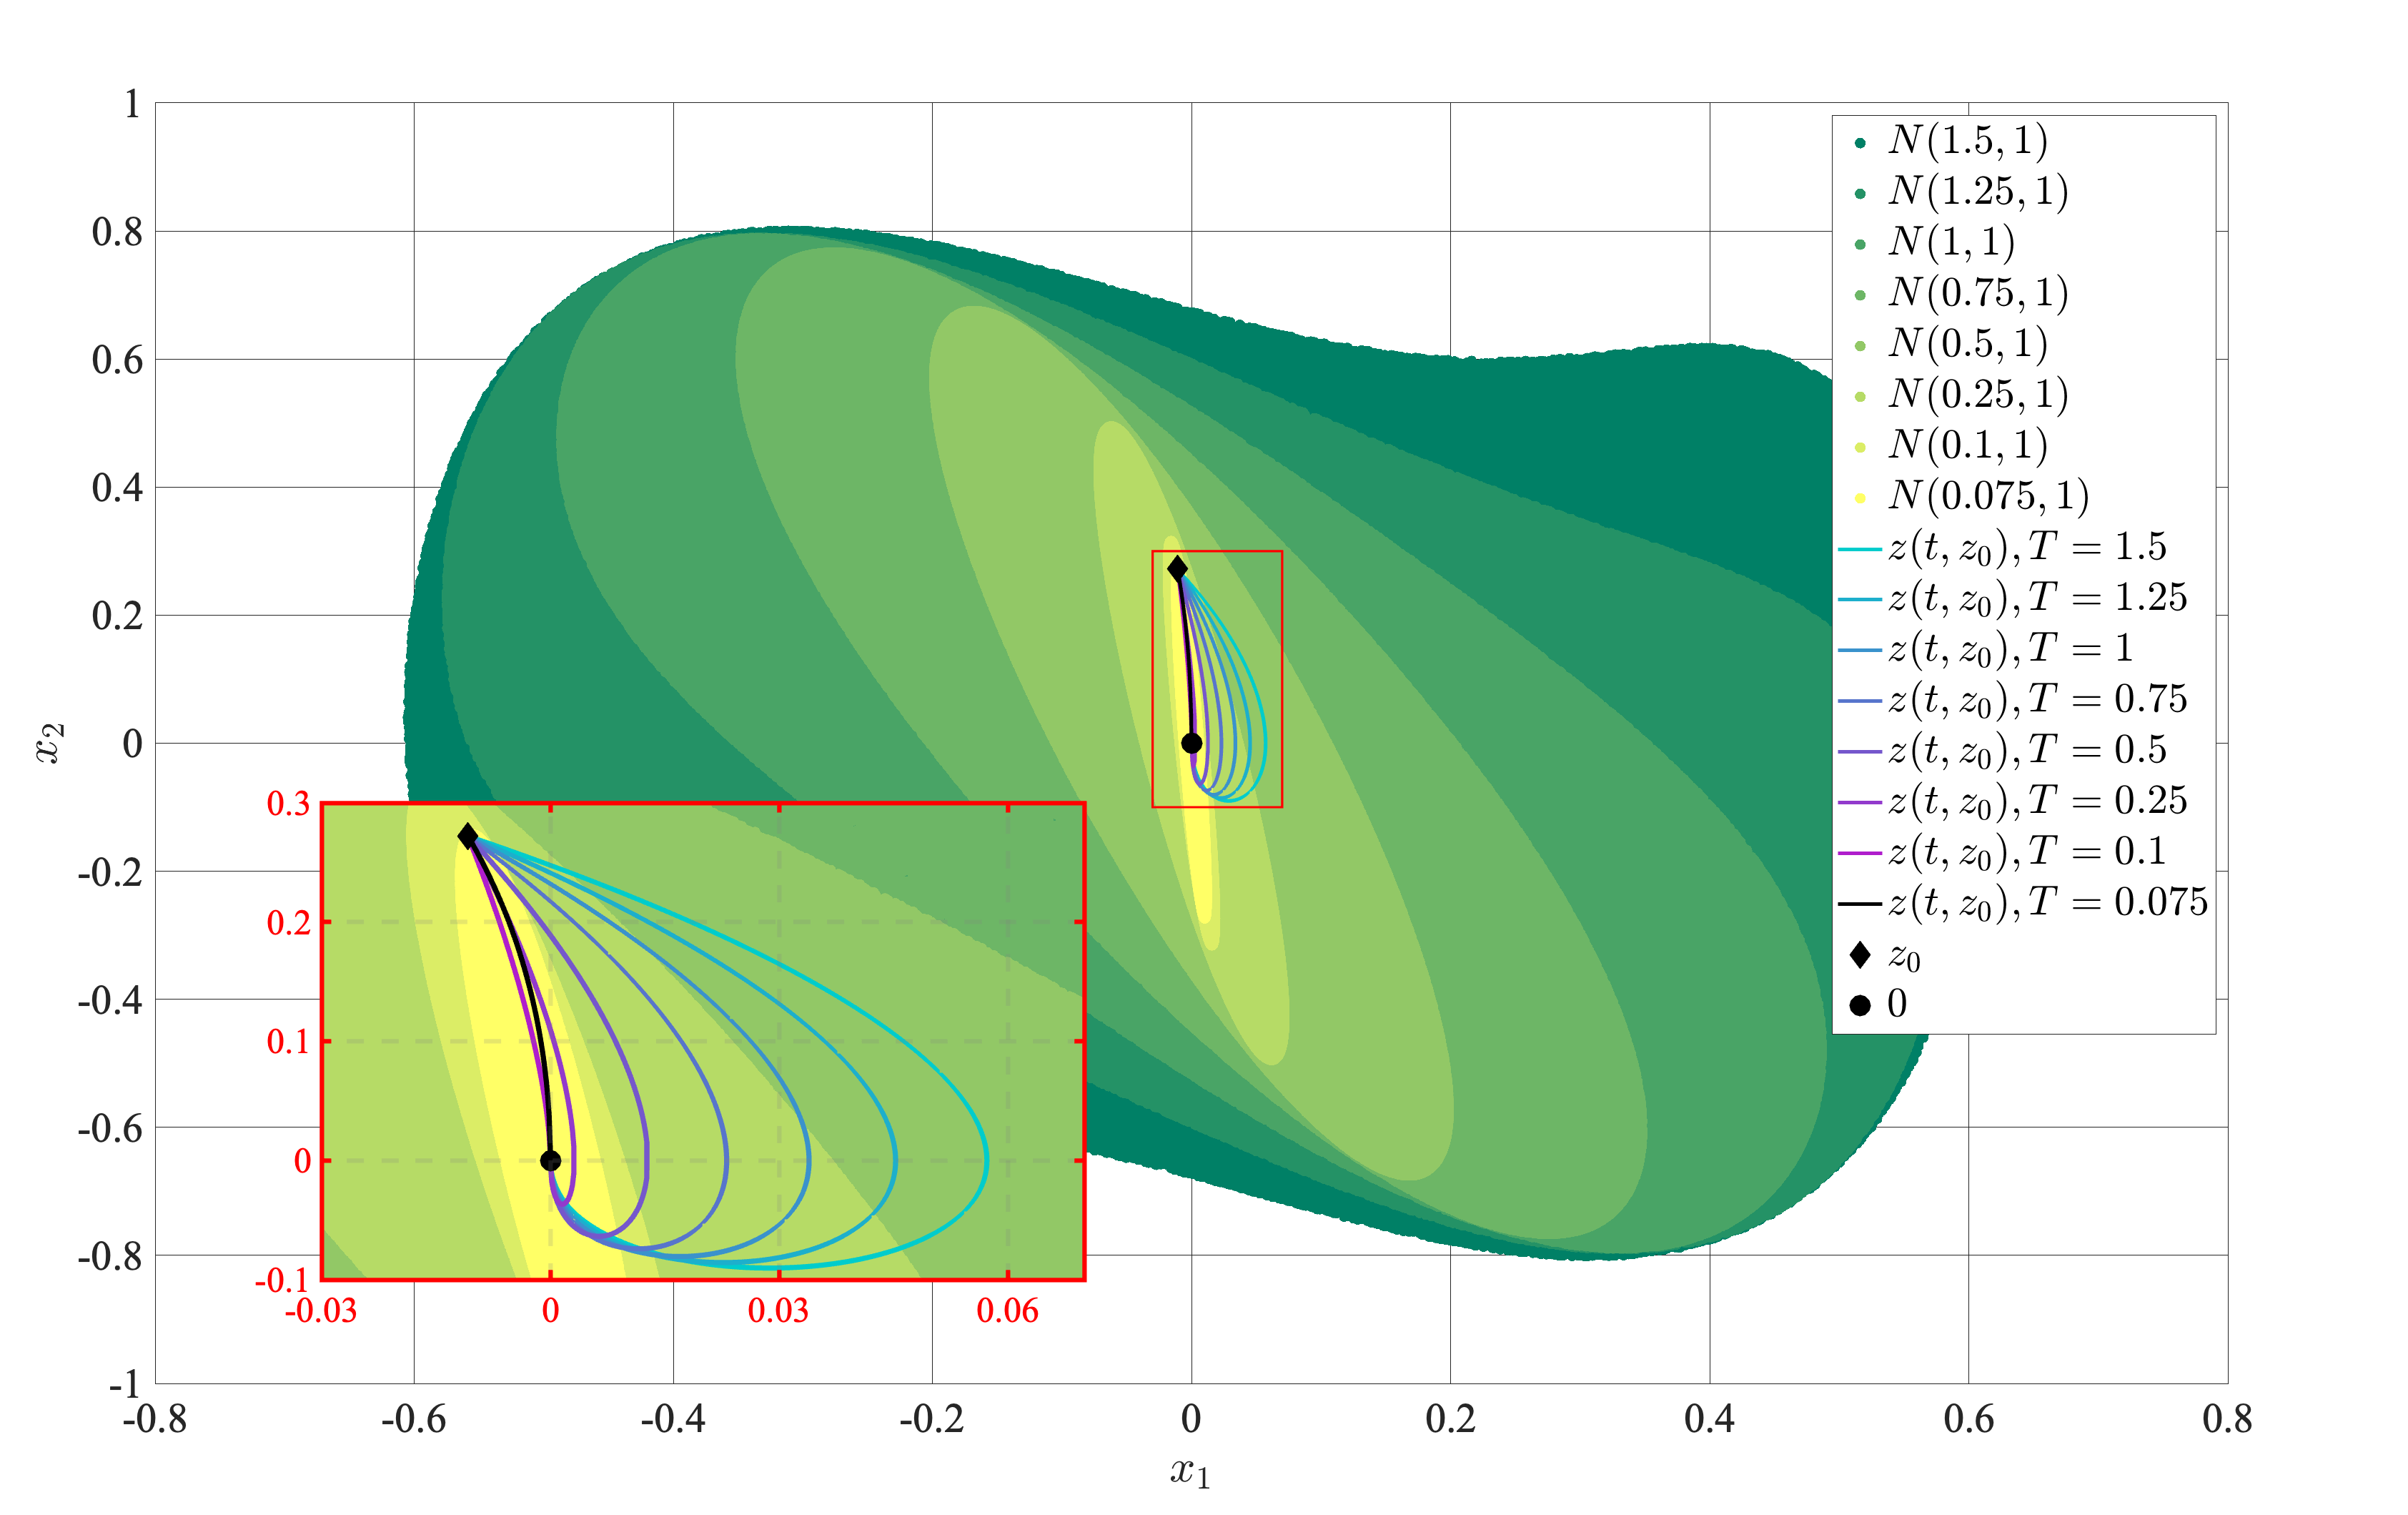
\includegraphics[width=\linewidth]{images/GusevMIOsipov_Duffing_fixed_z0.eps}
 \caption{Результаты экспериментов с переменным $T$.}
 \label{s22:fig:series1}
\end{figure}

Несмотря на то, что условие $z_0 \in B(0,r_1(T))$ Теоремы \ref{s22:th:tends_to_zero} не выполняется при $r_1(T)$, используемом в доказательстве, траектории по-прежнему стремятся к нулю. 
Это можно объяснить слишком строгим выбором $r_1(T)$ и тем, что теорема \ref{s22:th:tends_to_zero} формулирует только достаточные условия для того, чтобы траектории стремились к нулю. 
Можно заметить, что в случае фиксированных начальных условий с уменьшением $T$ относительная разность функционалов $\Delta_J$ уменьшается, что следует из оценки, полученной в теореме \ref{s22:th:functional_error_estimate}.

Теперь немного изменим условия эксперимента. 
Мы изменим не только $T$, но и начальные условия $z_0$ так, чтобы, во-первых, выполнялось равенство 
$z_0^{\top} Q_T(0) z_0 = 1$, а во-вторых, чтобы точка $z_0$ находилась внутри 
соответствующего множества нуль-управляемости $G_{-}(T,1)$.


\begin{table}
\caption{Результаты экспериментов с изменением $T$ и $z_0$}
\label{s22:ExampleTable2}
\begin{center}
\begin{tabular}{c|c|c|c|c|c|c}
 № & $T$ & $z_0$ & $\|z_0\|^2$&$z_0^{\top} Q_T(0) z_0$ &$J(T,z_0)$&$\Delta_J$ \\ \hline 
 1 & 1.500 & [-0.594;-0.057] & 0.356680 & 0.999993 & 1.075833 & 0.0758407 \\ \hline
 2 & 1.250 & [-0.578;0.226] & 0.385032 & 0.999997 & 1.110464 & 0.1104671 \\ \hline
 3 & 1.000 & [-0.502;0.508] & 0.509514 & 0.999999 & 1.108159 & 0.1081607 \\ \hline
 4 & 0.750 & [-0.354;0.652] & 0.550391 & 1.000000 & 1.048784 & 0.0487844 \\ \hline
 5 & 0.500 & [-0.195;0.638] & 0.445513 & 1.000000 & 1.009848 & 0.0098475 \\ \hline
 6 & 0.250 & [-0.069;0.481] & 0.236487 & 1.000000 & 1.000349 & 0.0003490 \\ \hline
\end{tabular}
\end{center}
\end{table} 

Результаты этой серии экспериментов 
показаны на Рисунке \ref{s22:fig:series2} и в Таблице 
\ref{s22:ExampleTable2}.
Зелёными областями обозначены множества нуль-управляемости $G_{-}(T,1)$ системы 
\eqref{s22:Duffing} при $T = \{0.25, 0.5, 0.75, 1.0, 1.25, 1.5\}$, пунктирные линии показывают границы множества нуль-управляемости линеаризованной системы 
\eqref{s22:LinearDuffing}, сплошные линии показывают траектории нелинейной системы 
при различных $T$. 
Символы "$\blacklozenge$" разных цветов обозначают 
начальные условия $z_0$, а "$\bullet$" --- целевую точку, расположенную в начале координат. 

Замечание о невыполнении условия из первой части примера актуально и здесь. 
Из Таблицы \ref{s22:ExampleTable2} видно, что значения $\Delta_J$ также уменьшаются с уменьшением $T$, но это уменьшение не монотонно. 
По-видимому, это связано с тем, что меняется не только $T$, но и $z_0$.

\begin{figure}
 \centering
 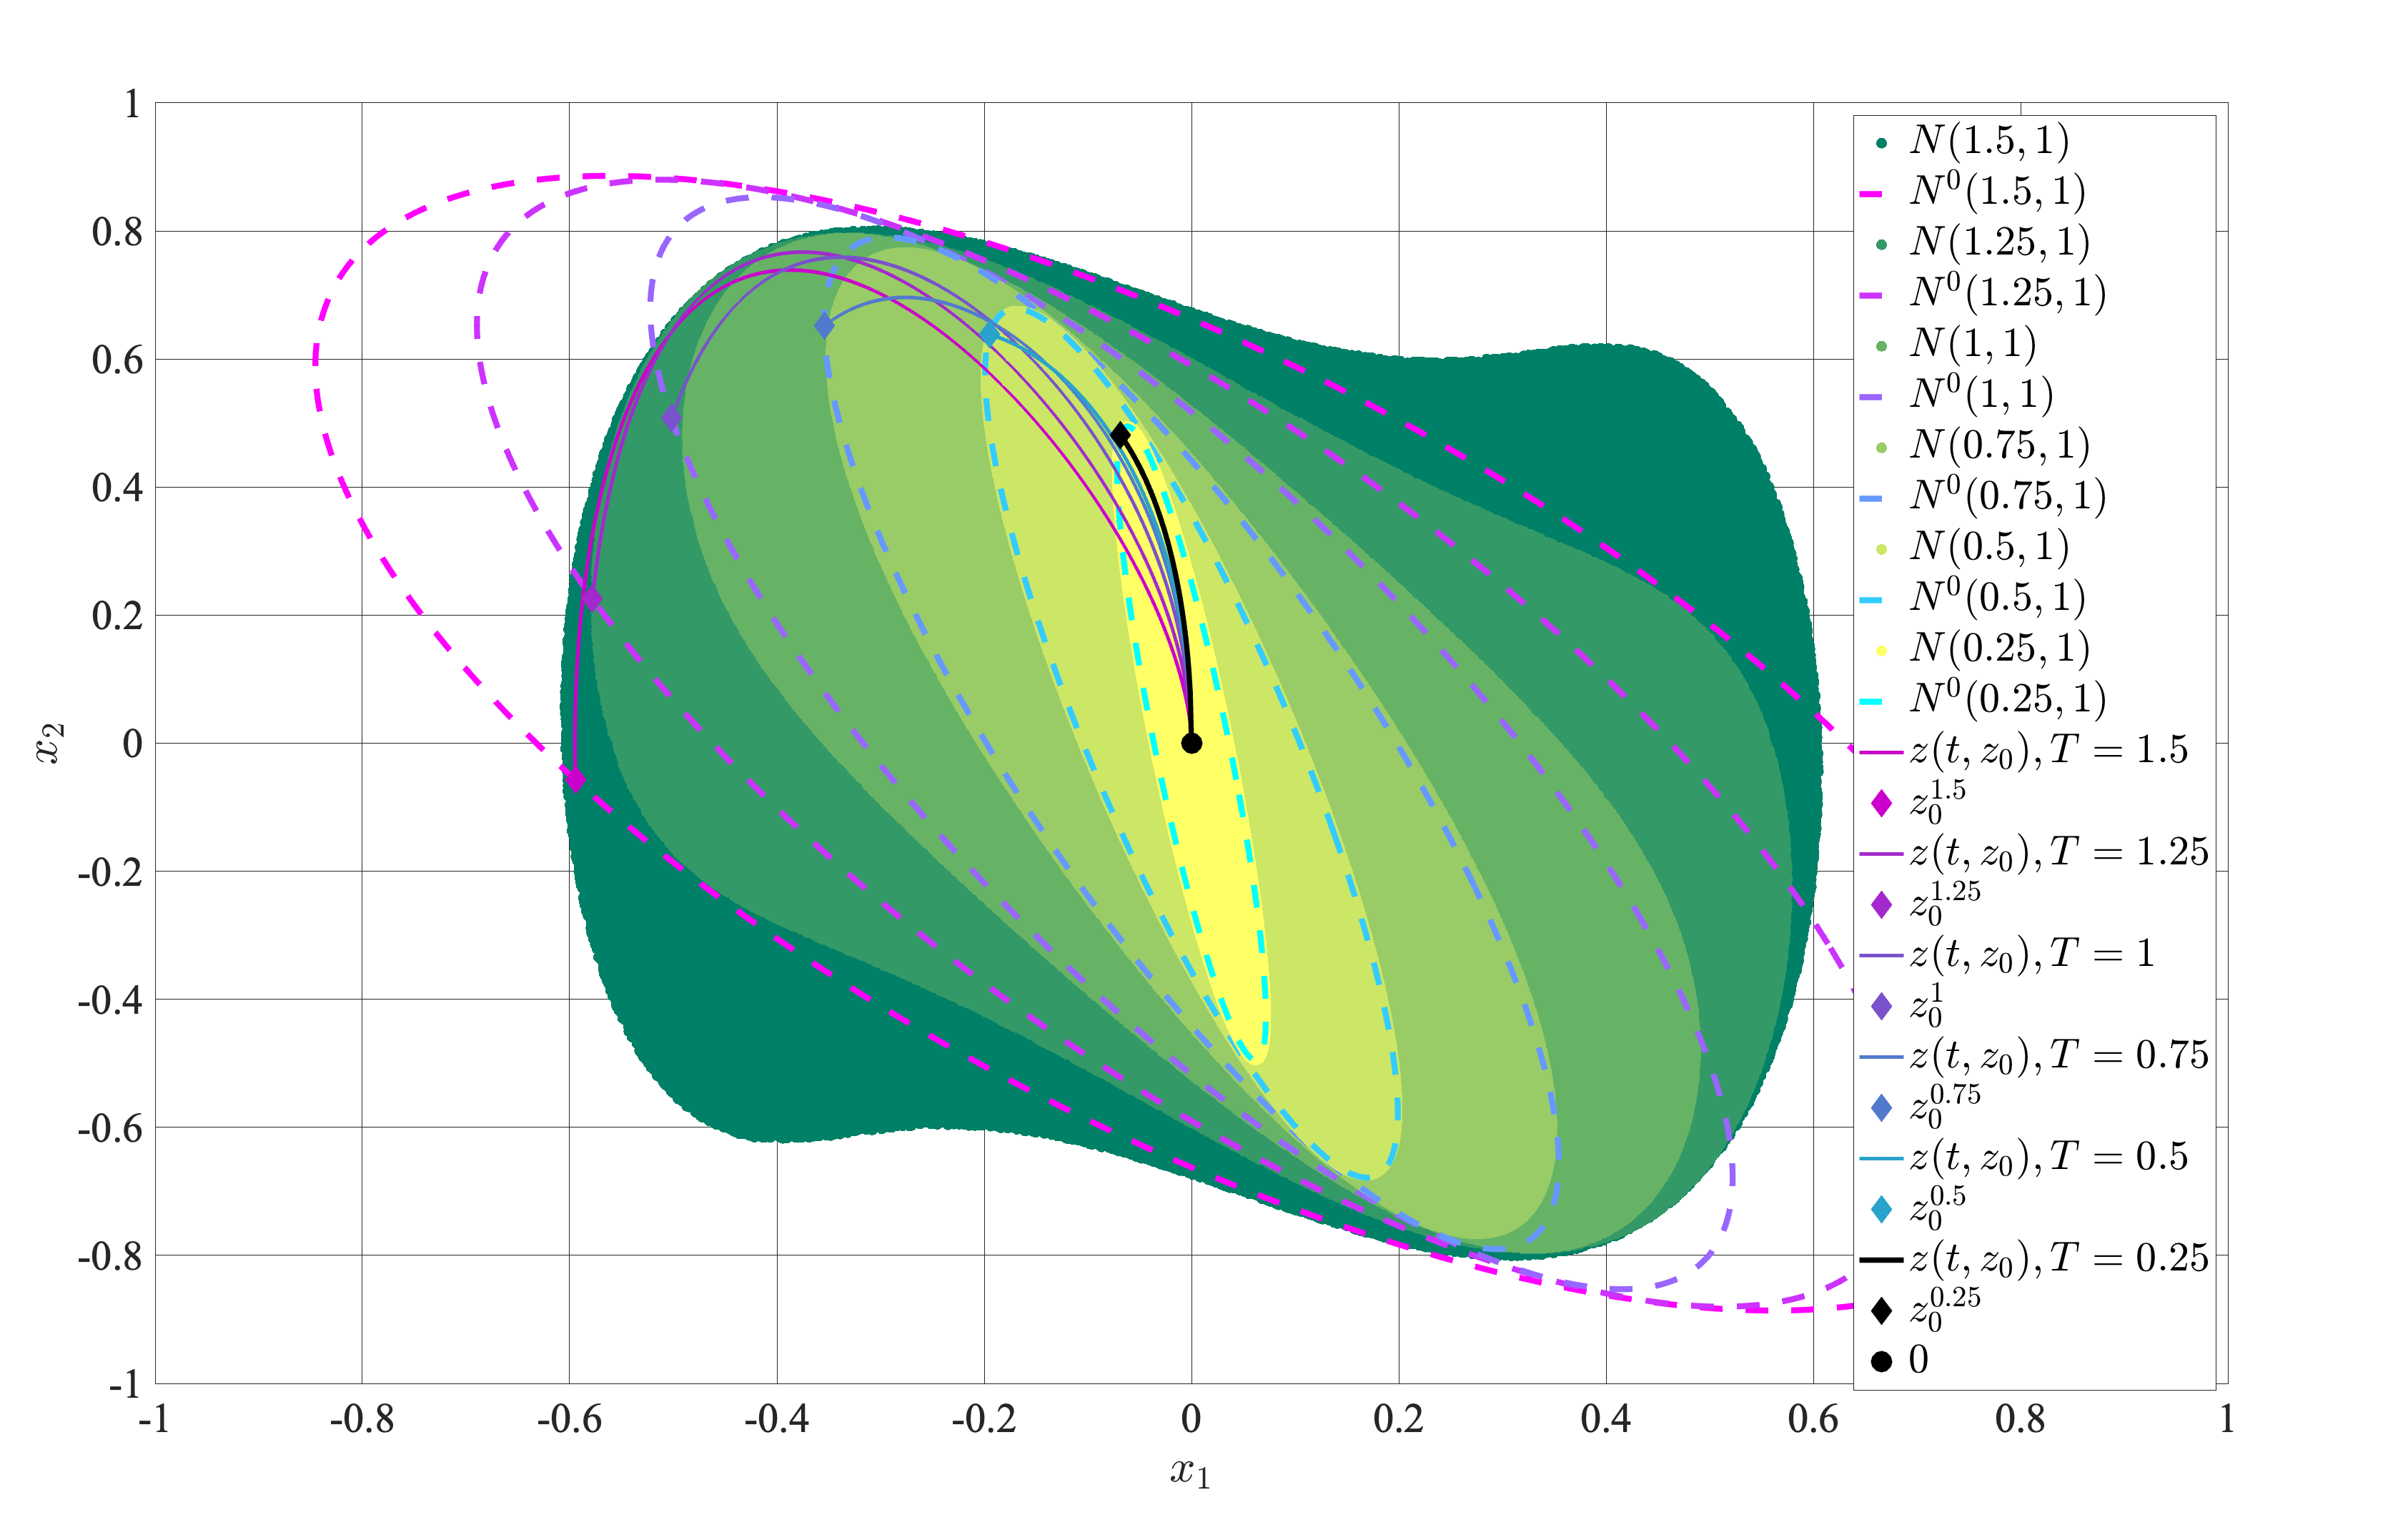
\includegraphics[width=\linewidth]{images/GusevMIOsipov_Duffing_variable_z0.eps}
 \caption{Результаты экспериментов с изменением $T$ и $z_0$}
 \label{s22:fig:series2}
\end{figure}

Также на Рисунке \ref{s22:fig:series2} видно, что множества нуль-управляемости нелинейной и линеаризованной систем близки по форме при $ T \leqslant 0.75$.

\end{document}